\documentclass{article}
\usepackage[utf8]{inputenc}
\usepackage[T1]{fontenc}
\usepackage{graphicx}
\usepackage{color}

\newenvironment{text-blue}{\color{blue}}{}
\newenvironment{text-red}{\color{red}}{}

\begin{document}

\title{Monitorização da temperatura do ar de um processo térmico \\ Trabalho prático nº3, Computação Adaptativa}
\author{Adriano Vinhas (2009106560, avinhas@student.dei.uc.pt)\\
		José Ribeiro (2008112181, jbaia@student.dei.uc.pt}
\maketitle
\clearpage

% Introdução
\section{Introdução}

\indent \indent Este trabalho, no âmbito da disciplina de Computação Adaptativa, tem como objectivo construir um sistema difuso capaz de regular a temperatura do ar através de um conjunto de entradas facultadas à rede, sendo estas alvo de transformação para corresponderem à lógica difusa. Estes valores vão ser a base da decisão de uma acção a tomar pelo sistema, que é feita através da saída.

Este objectivo foi atingido fazendo um estudo paramétrico tendo em conta os seguintes parâmetros de estudo:
\begin{itemize}
\item Factor de normalização
\item Conjunto e número de termos linguísticos
\item Tipo de funções de pertença
\item Base de regras
\item Mecanismo de inferência
\item Método de desfuzificação
\end{itemize}

A parte que foi mais focada na realização deste trabalho foi o estudo paramétrico feito com base nos parâmetros acima indicados. Com base nos resultados obtidos, procurámos uma solução que nos permitisse chegar à combinação dos parâmetros que minimizasse o erro da rede, para as referências que nos foram fornecidas.

\clearpage
\section{Concepção da rede difusa}
\indent \indent Nesta secção estão descritas a arquitectura da rede usada para o trabalho bem como outras decisões tomadas que são relevantes para o desempenho do controlador.

\subsection{Entradas}
\indent \indent A arquitectura do sistema difuso usada para o trabalho prático consiste em duas entradas, uma delas que representa o erro num instante $k$ ($E$) como a diferença entre a temperatura desejada e a temperatura do ar à saída do aquecedor nesse mesmo instante ($E = R_{k} - Y_{k}$), e a outra representando a variação do erro ($\Delta E$) como a diferença entre o erro no instante $k$ e $k-1$ ($\Delta E=E_{k}-E_{k-1}$).

Relativamente ao \textbf{universo de discurso}, considerámos que tanto as variáveis $E$ e $\Delta e$ tomariam valores entre -1 e 1, por serem valores \textit{default} usados para fins de normalização e no contexto do problema ser possível existir variações negativas ou positivas de temperatura.

Os valores de erro e variação de erro que serviram de entrada para o sistema de difuso foram alvos de normalização de modo a mapear os valores de temperatura e potência para valores correspondentes dentro do universo de discurso. Assim sendo, em relação aos \textbf{factores de normalização} utilizados, optámos por um usar um factor de escala de \textbf{0.02} para conseguir transformar a gama de valores de temperatura (entre 0 e 50ºC) no universo de discurso definido acima. Para o caso da potência, à saída, aplicou-se um factor de escala de \textbf{100} para fazer a transformação contrária e mapear valores do universo de discurso para a gama de valores que a potência pode tomar (entre 0 e 100\%). 

%Em relação às saídas do sistema difuso, apenas foi definida uma, que representa a variação de potência a aplicar à grelha de aquecimento ($\Delta U$).

%No que diz respeito às caracte

As restantes características da rede que são consideradas relevantes não são mencionadas aqui por terem sido alvo de estudo paramétrico.

A figura~\ref{nn_architecture} representa a arquitectura do sistema difuso usado.

\begin{figure}[!h]
  \centering
  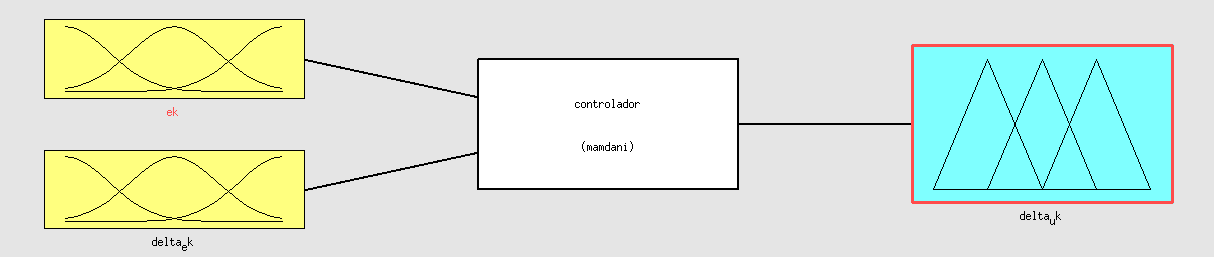
\includegraphics[width=5in]{figures/nn_architecture}
  \caption{Arquitectura da rede usada}
  \label{nn_architecture}
\end{figure}

O conjunto de regras que gerem as acções a tomar em função das entradas foi feito com especial cuidado uma vez que, entre outros factores, a definição das regras tem impacto na performance do sistema difuso.

O grupo decidiu implementar dois controladores que de seguida se apresentam.

\subsection{Controlador de 3 termos}
Para este controlador existem as três variáveis linguísticas mencionadas acima ($E$,$\Delta E$,$\Delta U$) e cada uma destas variavéis tem três termos linguísticos (${N,Z,P}$).

A tabela de regras para este controlador está representada na tabela~\ref{3_terms_fuzzy}.

\begin{table}[!h]
\centering
	\caption{Tabela de regras do controlador difuso de 3 termos}
	\label{3_terms_fuzzy}
	\begin{tabular}{|c|c|c|c|}
	\hline
	$E$ $\backslash$ $\Delta E$ & \textbf{N} & \textbf{ZO} & \textbf{P} \\ 
	\hline 
	\textbf{N} & N & N & ZO \\ 
	\hline 
	\textbf{ZO} & ZO & ZO & ZO \\ 
	\hline 
	\textbf{P} & ZO & P & P \\ 
	\hline 
	\end{tabular} 
	%\vspace{-1cm}
\end{table}

Esta tabela traduz-se na seguinte lista de regras:
\begin{itemize}
	\item \texttt{IF} <E \texttt{is} N> \texttt{AND} <$\Delta E$ \texttt{is} N> \texttt{THEN} <$\Delta U$ \texttt{is} N>
	\item \texttt{IF} <E \texttt{is} N> \texttt{AND} <$\Delta E$ \texttt{is} ZO> \texttt{THEN} <$\Delta U$ \texttt{is} N>
	\item \texttt{IF} <E \texttt{is} N> \texttt{AND} <$\Delta E$ \texttt{is} P> \texttt{THEN} <$\Delta U$ \texttt{is} ZO>
	\item \texttt{IF} <E \texttt{is} ZO> \texttt{AND} <$\Delta E$ \texttt{is} N> \texttt{THEN} <$\Delta U$ \texttt{is} ZO>
	\item \texttt{IF} <E \texttt{is} ZO> \texttt{AND} <$\Delta E$ \texttt{is} ZO> \texttt{THEN} <$\Delta U$ \texttt{is} ZO>
	\item \texttt{IF} <E \texttt{is} ZO> \texttt{AND} <$\Delta E$ \texttt{is} P> \texttt{THEN} <$\Delta U$ \texttt{is} ZO>
	\item \texttt{IF} <E \texttt{is} P> \texttt{AND} <$\Delta E$ \texttt{is} N> \texttt{THEN} <$\Delta U$ \texttt{is} ZO>
	\item \texttt{IF} <E \texttt{is} P> \texttt{AND} <$\Delta E$ \texttt{is} ZO> \texttt{THEN} <$\Delta U$ \texttt{is} P>
	\item \texttt{IF} <E \texttt{is} P> \texttt{AND} <$\Delta E$ \texttt{is} P> \texttt{THEN} <$\Delta U$ \texttt{is} P>
\end{itemize}

\clearpage

\subsection{Controlador de 5 termos}
Para este controlador existem as mesmas variáveis linguísticas e cada uma destas variavéis tem cinco termos linguísticos (${NG,NP,ZO,PP,PG}$).

A tabela de regras para este controlador está representada na tabela~\ref{5_terms_fuzzy}.

\begin{table}[!h]
\centering
	\caption{Tabela de regras do controlador difuso de 5 termos}
	\label{5_terms_fuzzy}
	\begin{tabular}{|c|c|c|c|c|c|}
	\hline
	$E$ $\backslash$ $\Delta E$ & \textbf{NG} & \textbf{NP} & \textbf{ZO} & \textbf{PP} & \textbf{PG} \\ 
	\hline 
	\textbf{NG} & NG & NG & NG & NP & NP \\ 
	\hline 
	\textbf{NP} & NP & NP & NP & NP & NG \\ 
	\hline 
	\textbf{ZO} & NP & ZO & ZO & ZO & PP \\ 
	\hline
	\textbf{PP} & PG & PP & PP & PP & PP \\ 
	\hline 
	\textbf{PG} & PP & PP & PG & PG & PG \\ 
	\hline 
	\end{tabular} 
	%\vspace{-1cm}
\end{table}

Esta tabela traduz-se na seguinte lista de regras:
\begin{itemize}
	\item \texttt{IF} <E \texttt{is} NG> \texttt{AND} <$\Delta E$ \texttt{is} NG> \texttt{THEN} <$\Delta U$ \texttt{is} NG>
	\item \texttt{IF} <E \texttt{is} NG> \texttt{AND} <$\Delta E$ \texttt{is} NP> \texttt{THEN} <$\Delta U$ \texttt{is} NG>
	\item \texttt{IF} <E \texttt{is} NG> \texttt{AND} <$\Delta E$ \texttt{is} ZO> \texttt{THEN} <$\Delta U$ \texttt{is} NG>
	\item \texttt{IF} <E \texttt{is} NG> \texttt{AND} <$\Delta E$ \texttt{is} PP> \texttt{THEN} <$\Delta U$ \texttt{is} NP>
	\item \texttt{IF} <E \texttt{is} NG> \texttt{AND} <$\Delta E$ \texttt{is} PG> \texttt{THEN} <$\Delta U$ \texttt{is} NP>
	\item \texttt{IF} <E \texttt{is} NP> \texttt{AND} <$\Delta E$ \texttt{is} NG> \texttt{THEN} <$\Delta U$ \texttt{is} NP>
	\item \texttt{IF} <E \texttt{is} NP> \texttt{AND} <$\Delta E$ \texttt{is} NP> \texttt{THEN} <$\Delta U$ \texttt{is} NP>
	\item \texttt{IF} <E \texttt{is} NP> \texttt{AND} <$\Delta E$ \texttt{is} ZO> \texttt{THEN} <$\Delta U$ \texttt{is} NP>
	\item \texttt{IF} <E \texttt{is} NP> \texttt{AND} <$\Delta E$ \texttt{is} PP> \texttt{THEN} <$\Delta U$ \texttt{is} NP>
	\item \texttt{IF} <E \texttt{is} NP> \texttt{AND} <$\Delta E$ \texttt{is} PG> \texttt{THEN} <$\Delta U$ \texttt{is} NG>
	\item \texttt{IF} <E \texttt{is} ZO> \texttt{AND} <$\Delta E$ \texttt{is} NG> \texttt{THEN} <$\Delta U$ \texttt{is} NP>
	\item \texttt{IF} <E \texttt{is} ZO> \texttt{AND} <$\Delta E$ \texttt{is} NP> \texttt{THEN} <$\Delta U$ \texttt{is} ZO>
	\item \texttt{IF} <E \texttt{is} ZO> \texttt{AND} <$\Delta E$ \texttt{is} ZO> \texttt{THEN} <$\Delta U$ \texttt{is} ZO>
	\item \texttt{IF} <E \texttt{is} ZO> \texttt{AND} <$\Delta E$ \texttt{is} PP> \texttt{THEN} <$\Delta U$ \texttt{is} ZO>
	\item \texttt{IF} <E \texttt{is} ZO> \texttt{AND} <$\Delta E$ \texttt{is} PG> \texttt{THEN} <$\Delta U$ \texttt{is} PP>
	\item \texttt{IF} <E \texttt{is} PP> \texttt{AND} <$\Delta E$ \texttt{is} NG> \texttt{THEN} <$\Delta U$ \texttt{is} PG>
	\item \texttt{IF} <E \texttt{is} PP> \texttt{AND} <$\Delta E$ \texttt{is} NP> \texttt{THEN} <$\Delta U$ \texttt{is} PP>
	\item \texttt{IF} <E \texttt{is} PP> \texttt{AND} <$\Delta E$ \texttt{is} ZO> \texttt{THEN} <$\Delta U$ \texttt{is} PP>
	\item \texttt{IF} <E \texttt{is} PP> \texttt{AND} <$\Delta E$ \texttt{is} PP> \texttt{THEN} <$\Delta U$ \texttt{is} PP>
	\item \texttt{IF} <E \texttt{is} PP> \texttt{AND} <$\Delta E$ \texttt{is} PG> \texttt{THEN} <$\Delta U$ \texttt{is} PP>
	\item \texttt{IF} <E \texttt{is} PG> \texttt{AND} <$\Delta E$ \texttt{is} NG> \texttt{THEN} <$\Delta U$ \texttt{is} PP>
	\item \texttt{IF} <E \texttt{is} PG> \texttt{AND} <$\Delta E$ \texttt{is} NP> \texttt{THEN} <$\Delta U$ \texttt{is} PP>
	\item \texttt{IF} <E \texttt{is} PG> \texttt{AND} <$\Delta E$ \texttt{is} ZO> \texttt{THEN} <$\Delta U$ \texttt{is} PG>
	\item \texttt{IF} <E \texttt{is} PG> \texttt{AND} <$\Delta E$ \texttt{is} PP> \texttt{THEN} <$\Delta U$ \texttt{is} PG>
	\item \texttt{IF} <E \texttt{is} PG> \texttt{AND} <$\Delta E$ \texttt{is} PG> \texttt{THEN} <$\Delta U$ \texttt{is} PG>
\end{itemize}

\clearpage
% Gráficos com os resultados. Análise e interpretação.
\section{Estudo paramétrico}
\indent \indent Nesta secção é explicada a metodologia de testes seguida para levar a cabo são apresentados os resultados do estudo paramétrico efectuado para obtenção do resultado óptimo encontrado.

Neste estudo, a ordem dos parâmetros testados torna-se fulcral para melhor explorar o espaço de combinações sem o fazer de forma exaustiva. No fim de cada variação paramétrica, o valor que optimizava as métricas usadas para medir a performance da rede neuronal era fixado na variação paramétrica seguinte. Por exemplo, após a determinação do número óptimo de neurónios para a camada escondida, esse valor era fixado para os restantes testes.

No caso do estudo do coeficiente de aprendizagem, tal não se aplica uma vez que este foi o 
\begin{table}[!h]
\centering
	\caption{Tabela de regras do controlador difuso de 5 termos}
	\label{results}
	\begin{tabular}{|c|c|c|c|c|c|}
		\hline 
		\textbf{Nº de termos} & \textbf{Funções} & \textbf{Operadores} & \textbf{Desfuzificação} & \textbf{Média} & \textbf{Desvio-Padrão} \\
		\hline
		3 terms & \texttt{trimf} & \texttt{algebraic} & \texttt{centroid} & 86.627 & 3.624 \\
		\hline
		3 terms & \texttt{trimf} & \texttt{algebraic} & \texttt{bisector} & 83.846 & 2.199 \\
		\hline
		3 terms & \texttt{trimf} & \texttt{zadeh} & \texttt{centroid} & 74.824 & 0.593 \\
		\hline
		3 terms & \texttt{trimf} & \texttt{zadeh} & \texttt{bisector} & 74.204 & 0.652 \\
		\hline
		3 terms & \texttt{gauss} & \texttt{algebraic} & \texttt{centroid} & 73.320 & 0.499 \\
		\hline
		3 terms & \texttt{gauss} & \texttt{algebraic} & \texttt{bisector} & 85.331 & 3.419 \\
		\hline
		3 terms & \texttt{gauss} & \texttt{zadeh} & \texttt{centroid} & 73.121 & 0.574 \\
		\hline
		3 terms & \texttt{gauss} & \texttt{zadeh} & \texttt{bisector} & 73.377 & 0.464 \\
		\hline
		5 terms & \texttt{trimf} & \texttt{algebraic} & \texttt{centroid} & 107.419 & 0.79 \\
		\hline
		5 terms & \texttt{trimf} & \texttt{algebraic} & \texttt{bisector} & 108.633 & 1.591 \\
		\hline
		5 terms & \texttt{trimf} & \texttt{zadeh} & \texttt{centroid} & 103.604 & 0.813 \\
		\hline
		5 terms & \texttt{trimf} & \texttt{zadeh} & \texttt{bisector} & 104.01 & 1.747 \\
		\hline
		5 terms & \texttt{gauss} & \texttt{algebraic} & \texttt{centroid} & 100.416 & 0.516 \\
		\hline
		5 terms & \texttt{gauss} & \texttt{algebraic} & \texttt{bisector} & 114.191 & 0.947 \\
		\hline
		5 terms & \texttt{gauss} & \texttt{zadeh} & \texttt{centroid} & 93.625 & 0.525 \\
		\hline
		5 terms & \texttt{gauss} & \texttt{zadeh} & \texttt{bisector} & 106.071 & 1.7 \\
		\hline
	\end{tabular} 
	%\vspace{-1cm}
\end{table}

\clearpage
\section{Conclusão}
\indent \indent Depois do estudo paramétrico efectuado o sistema difuso que obteve melhores resultados tinha um valor de erro/critério de \textbf{xxx}, para a entrada que nos foi fornecida para efeitos de avaliação.

Atingimos estes valores usando a seguinte parametrização:
\begin{itemize}
\item Número de termos linguísticos:
\item Tipo de funções de pertença:
\item Factores de Normalização:
\item xxx
\item yyy
\item zzz
%\item Goal (Erro de treino) ???
\end{itemize}

O gráfico que representa os valores da referência, temperatura e controlo, para o melhor sistema difuso obtido, está exibido na figura ~\ref{best_fuzzy_results}. Os valores de entrada que nos foram fornecidos tiveram em conta um intervalo de tempo de 10 segundos e um intervalo de amostragem de 0.1s.
%\begin{figure}[h!]
%  \centering
%  \includegraphics[width=5in]{figures/best_nn}
%  \caption{Performance, Sensibilidade e Especificidade da melhor rede encontrada}
%  \label{best_nn}
%\end{figure}


\end{document}
